\documentclass[a4paper]{article}
\usepackage[margin=1in]{geometry}
\usepackage{titlesec}
\usepackage{enumitem}
\usepackage{parskip}
\usepackage{lmodern}
\usepackage{graphicx}
\usepackage{wrapfig}
\usepackage{multicol}
\usepackage{lipsum}
\usepackage{tabularx} 
\usepackage{array}
\parskip 1ex


\begin{document}
\thispagestyle{empty}

% Title & Subtitle with Image on Right
\begin{center}
    {\Large \textbf{Path Planning Algorithm for Automated Fiber Placement}}\\[0.1em]
    \hfill
   % \includegraphics[width=3cm]{image1.jpg} % Replace with actual image file
\end{center}


\vspace{1em}
\hrule
\vspace{1em}


\begin{tabularx}{\textwidth}{>{\centering\arraybackslash}X>{\centering\arraybackslash}X>{\centering\arraybackslash}X}
    \textbf{Role} & \textbf{Organization} & \textbf{Date} \\
    Robotics Engineer Intern & SIT Prototype Object Fabrication Lab & May 2024 - Dec 2024 
\end{tabularx}

% Body Section: What I did with Image on Left
\section*{What I did}

\noindent
\parbox[b]{.6\textwidth}{
    Utilized OpenCV and computer vision techniques to map the robot's workspace.
    Created a virtual testing environment for the DOOSAN H2515 collaborative robot using MATLAB and ROS 2.0.
    Designed a 3D model of the roller end-effector in SolidWorks and developed the PCB in C++.

}
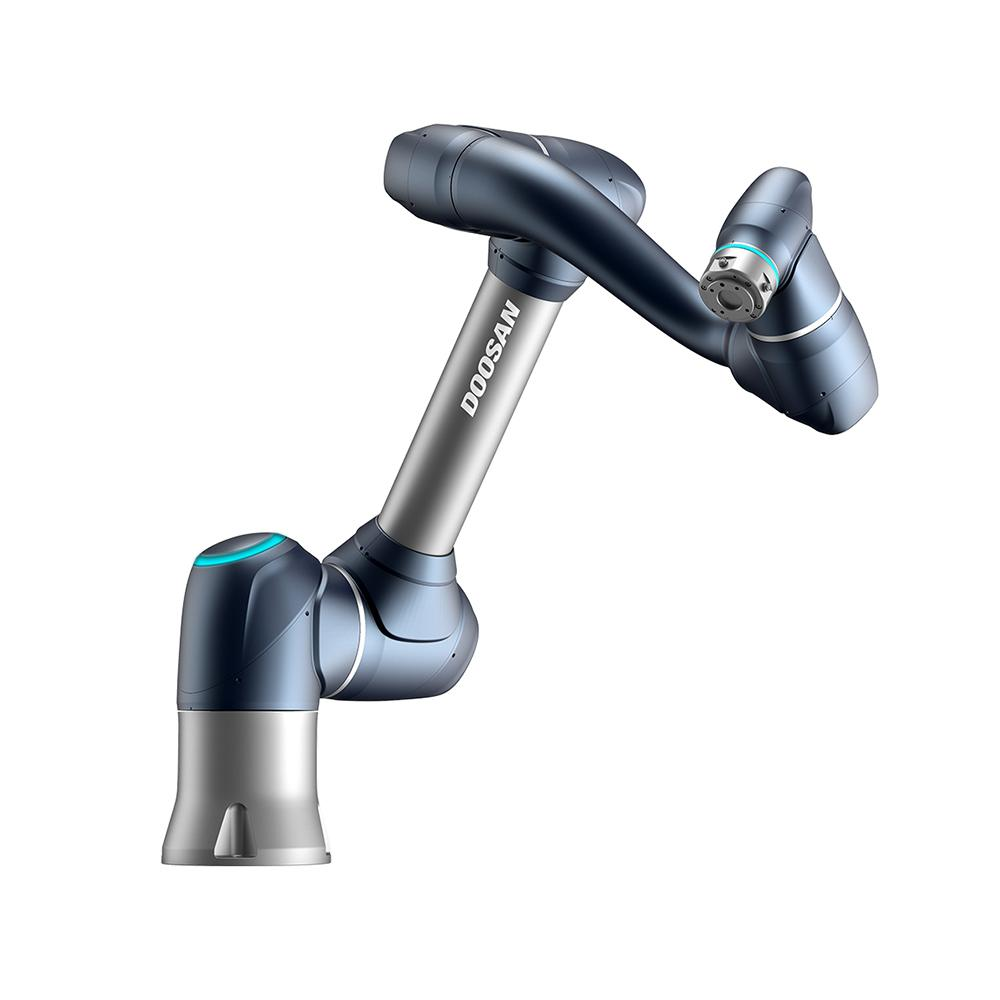
\includegraphics[width=.4\textwidth]{images/doosan-logo.jpg}%

% Body Section: How I did it with Image on Right

\noindent

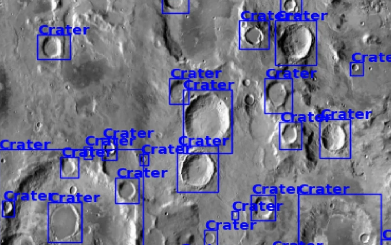
\includegraphics[width=.4\textwidth]{images/img-processing.png}
\parbox[b]{.6\textwidth}{
    \textbf{How I did it} \\
    Utilized OpenCV and omputer vision techniques to map the robot's workspace.
    Created a virtual testing environment for the DOOSAN H2515 collaborative robot using MATLAB and ROS 2.0.
    Designed a 3D model of the roller end-effector in SolidWorks and developed the PCB in C++.

}
% Body Section: Tools/Environment and Results
\section*{Tools \& Results}
\textbf{Tools/Environments:}
\begin{itemize}[leftmargin=*, noitemsep]
    \item DOOSAN H2125 collaborative robot.
    \item MATLAB simulation environment.
\end{itemize}

\vspace{0.5em}
\textbf{Results:}
\begin{itemize}[leftmargin=*, noitemsep]
    \item Successfully developed a Path Planning Algorithm for Automatic Fiber Placement.
    \item Enhanced lab operations with improved algorithm efficiency and reliability.
    \item Reduced testing time and costs by using the virtual environment.
\end{itemize}

\vfill
\hrule
\vspace{0.5em}

% Special Skills Section
\section*{Special Skills}
\begin{itemize}[leftmargin=*, noitemsep]
    \item MATLAB \& ROS 2.0 Development
    \item OpenCV \& Computer Vision Mapping
    \item Python Programming for Path Planning
    \item SolidWorks 3D Modeling
    \item PCB Design and C++ Programming
\end{itemize}



% Four-Column Skills Table
\noindent
\begin{tabularx}{\textwidth}{|>{\centering\arraybackslash}X|>{\centering\arraybackslash}X|>{\centering\arraybackslash}X|>{\centering\arraybackslash}X|}

    Robotics & Machine Learning & Control Systems & Embedded Systems \\ 
    3D CAD Modeling & Computer Vision & Image Processing & Artificial Intelligence \\ 
    Sensor Fusion & Optimization & Signal Processing & AutomationEngineering \\ 
    MATLAB & Python Programming & ROS 2.0 & PCB Design \\ 
\end{tabularx}



    


\end{document}
